\chapter{Experimental Setup}
The 2 sister experiments were carried out in Hall A of Jlab, 

% table of beam parameters
\begin{table}[h]
    \centering
    \begin{tabular}{c | c c }
	\hline
	&   PREX-II & CREX  \\
	\hline
	Target	& \Pb	& \Ca	\\
	Target thickness (mm)	& 0.5	& 6	\\
	\hline
	Beam Energy ($GeV$) & 0.97 & 2.18  \\
	Beam Current ($\mu A$)	& 70	& 150	\\
	Beam Polarization & 88\%   & 87.1\%   \\
	Scattering angle ($\deg$)   & 5	& 4.51 \\
	$Q^2$ ($GeV^2$)	&   & 0.0297	\\
	Helicity rate (Hz)  & 240   & 120   \\
	rate/arm (MHz)	&   & 25    \\
	\hline
    \end{tabular}
\end{table}

%%%%%%%%%%%%%%%%%%%%%%%%%%%%%%%%%%%%%%%%%%%%%%%%
\subsection{Design}
Though weak charge distribution is what we want to measure, it doesn't mean we
know nothing about it. Due to the symmetry between proton and neutron, we would
expect the weak charge (neutron) distribution is similar to the charge (proton)
distribution. Based on this assumption, we will have some models to describe
the neutron distribution and therefore the FFs, from which we can derive the
cross section and their asymmetry.

For symmetric nuclei with equal number of proton and neutron, it is expected 
that their density distributions are similar to each other, which are usually
expressed as a 2-parameter Fermi function:
\begin{equation}
    \rho(r) = \frac{\rho_0}{1 + exp(r-a)/c}
\end{equation}
where a and c denote the half-height radius and diffuseness respectively. 
% Thiel et al J.Phys.G 46 (2019) 9, 093003 

\subsubsection{Sensitivity}

%%%%%%%%%%%%%%%%%%%%%%%%%%%%%%%%%%%%%%%%%%%%%%%%
\subsection{Continuous Electron Beam Accelerator Facility (CEBAF)}
\begin{figure}[h]
    \includegraphics[width=0.5\linewidth]{jlab_1.jpg}
    \caption{aerial view of CEBAF} 
\end{figure}
\begin{figure}[h]
    \includegraphics[width=0.9\linewidth]{cebaf.png}
    \caption{Schematic plot of CEBAF: Hall D don't have its own slot, so it 
    follows either A or C} 
\end{figure}
With the 12 GeV upgrade, the north and south LINAC each has 25 cryomodules, 
capable of accelrating electrons at the rate of 2.2 $GeV/turn$. The special
design of CEBAF allows it to deliver electron beams of different energies to
3 (4) halls simultaneously, as long as the total beam power is less than 1 MW.
So different nuclear experiments can be carried out in different halls at the 
same time.

%%%%%%%%%%%%%%%%%%%%%%%%%%%%%%%%%%%%%%%%%%%%%%%%
\subsection{Polarized Electron Source}
PVES experiments motivate the development of polarized electron source, which 
require a highly stable polarized electron source that can produce
high polarization electron beam at a wide range of intensity, from nA to A 
depending on the experiment. The source should be capable of rapid helicity
reversal ($\sim 100 Hz$) with negligible impact on other properties of the beam.

Currently, GaAs-based semiconductor photoemission source is % confirmed by Wang Yan
the only available polarized electron source for accelerators on the market.
Historically, this 
kind of electron source was the only one that could satisfy high peak currents 
required by the low duty factors of the old accelerators and rapid helicity 
reversal required by PVES. That's why it is the only player on the market now.
Over the past few decades, pulsed beam has been replaced by continuous beam while
this electron source is inheritated and further developed. The polarized electron
source used by CEBAF can produce electron beam with polarization greater than
85\%, much larger than the 37\% polarization from its inauguration at SLAC. \cite{PRESCOTT1978347}

The design was first proposed independently by Garwin, Pierce and Siegmann \cite{GARWIN}
and by Lampel and Weisbuch \cite{LAMPEL1975877}. The idea is straightforward:
When circularly polarized laser light with carefully selected energy $E_{gap} < h\nu < E_{gap} + \Delta$
shoot on the semiconductor, only electrons on the valance band $P_{3/2}$ will be
pumped into the conduction band $S_{1/2}$. The selection rule makes sure only
those transitions that satisfy $\Delta m_j = +1 \ (-1)$ can occur for circularly
right (left) incoming photons, As shown in fig. \ref{fg:excitation-b}.
The ratio of the transition rate is also marked out in circle in the plot, 
which can be calculated from the Clebsch-Gordan coefficient easily. The excited
electrons are polarzied and different states have different pumping rate, so
we have polarized electron beam now with polarization as: P = (3-1)/(3+1) = 50\%,
for both cases.
\begin{figure}[h]
    \tikzmath{\yone=1.3; \ytwo=2.5; \ythree=5;} 
    \centering
    \begin{subfigure}[b]{0.49\textwidth}
	\centering
	\begin{tikzpicture}
	    \centering
	    \begin{axis}[axis lines=middle,
		xmin=-1.4, xmax=2.75,
		ymin=0, ymax=7,
		xlabel={\large $k$},
		ylabel={\large$E$},
		xlabel style={below},
		xtick=\empty,
		ytick=\empty,
		x axis line style={draw=none},
		% clip=false,
		]
		\addplot[Violet, line width=3pt, samples=100, domain=-0.7:0.7, name path=A] {-2*x^2 + \yone};
		\addplot[OliveGreen, line width=3pt, samples=100, domain=-0.7:0.7, name path=B] {-2*x^2 + \ytwo};
		\addplot[OliveGreen, line width=3pt, samples=100, domain=-0.7:0.7, name path=B] {-1.2*x^2 + \ytwo};
		\addplot[Blue, line width=3pt, samples=100, domain=-0.7:0.7, name path=B] {2*x^2 + \ythree};
		\draw [/pgfplots/every inner x axis line, draw=black] (0,0) -- (\pgfkeysvalueof{/pgfplots/xmax}, 0); 
		\draw [dashed, draw=black] (0,\yone) -- (\pgfkeysvalueof{/pgfplots/xmax}, \yone);
		\draw [dashed, draw=black] (0,\ytwo) -- (\pgfkeysvalueof{/pgfplots/xmax}, \ytwo);
		\draw [dashed, draw=black] (0,\ythree) -- (\pgfkeysvalueof{/pgfplots/xmax}, \ythree);
		\draw [stealth-stealth, thick] (0.8, \yone) -- (0.8, \ytwo) node [midway, right] {\bm{$\Delta = 0.34\ eV$}};
		\draw [stealth-stealth, thick] (0.8, \ytwo) -- (0.8, \ythree) node [midway, right] {\bm{$E_{gap} = 1.42\ eV$}};
		\node [Violet, below] at (-1, \yone) {\large\bm{$P_{1/2}$}};
		\node [OliveGreen, below] at (-1, \ytwo) {\large\bm{$P_{3/2}$}};
		\node [Blue, above] at (-1, \ythree) {\large\bm{$S_{1/2}$}};
		\node [left, above] at (-0.2, \ytwo) {\large\bm{$E_F$}};
	    \end{axis}
	    \label{fg:excitation-a}
	\end{tikzpicture}
    \end{subfigure}
    \hfill
    \begin{subfigure}[b]{0.49\textwidth}
	\centering
	\begin{tikzpicture}
	    \begin{axis}[axis lines=middle,
		xmin=0, xmax=8,
		ymin=0, ymax=7,
		xlabel={\large $m_j$},
		ylabel={\large$E$},
		xlabel style={below},
		xtick=\empty,
		ytick=\empty,
		]
		\draw [/pgfplots/every inner y axis line, draw=black] (6.5,0) -- (6.5, \pgfkeysvalueof{/pgfplots/ymax}) node [below right] {\large J}; 
		\draw [draw=Violet, line width=2pt] (1.25,\yone) -- (2.25, \yone) node [midway, below, Violet] {\textbf{-1/2}};
		\draw [draw=Violet, line width=2pt] (4.25,\yone) -- (5.25, \yone) node [midway, below, Violet] {\textbf{+1/2}};
		\draw [draw=OliveGreen, line width=2pt] (0.5,\ytwo) -- (1.5, \ytwo) node [midway, below, OliveGreen] {\textbf{-3/2}};
		\draw [draw=OliveGreen, line width=2pt] (2,\ytwo) -- (3, \ytwo) node [midway, below, OliveGreen] {\textbf{-1/2}};
		\draw [draw=OliveGreen, line width=2pt] (3.5,\ytwo) -- (4.5, \ytwo) node [midway, below, OliveGreen] {\textbf{+1/2}};
		\draw [draw=OliveGreen, line width=2pt] (5,\ytwo) -- (6, \ytwo) node [midway, below, OliveGreen] {\textbf{+3/2}};
		\draw [draw=Blue, line width=2pt] (2,\ythree) -- (3, \ythree) node [midway, above, Blue] {\textbf{-1/2}};
		\draw [draw=Blue, line width=2pt] (3.5,\ythree) -- (4.5, \ythree) node [midway, above, Blue] {\textbf{+1/2}};
		\node [Violet, right] at (6.7, \yone-0.1) {\large\bm{$P_{1/2}$}};
		\node [OliveGreen, right] at (6.7, \ytwo-0.1) {\large\bm{$P_{3/2}$}};
		\node [Blue, right] at (6.7, \ythree-0.1) {\large\bm{$S_{1/2}$}};

		\draw [-stealth, Red, line width=2pt] (1, \ytwo) -- (2.5, \ythree) node [midway, circle, fill=CornflowerBlue, text=Black] {\textbf{3}};
		\draw [-stealth, Red, line width=2pt] (2.5, \ytwo) -- (4, \ythree);
		\node [above, Red] at (1, \ytwo+0.5) {\bm{$\sigma^+$}};
		\draw [-stealth, YellowOrange, line width=2pt] (4, \ytwo) -- (2.5, \ythree) node [midway, circle, fill=CornflowerBlue, text=Black] {\textbf{1}};
		\draw [-stealth, YellowOrange, line width=2pt] (5.5, \ytwo) -- (4, \ythree) node [midway, circle, fill=CornflowerBlue, text=Black] {\textbf{3}};
		\node [above, YellowOrange] at (5.5, \ytwo+0.5) {\bm{$\sigma^-$}};
	    \end{axis}
	\end{tikzpicture}
	\label{fg:excitation-b}
    \end{subfigure}
    \caption{Excitation of polarized electrons}
\end{figure}

\begin{figure}
    \centering
    \begin{subfigure}[b]{0.32\textwidth}
	\tikzmath{\yone=2.5; \ytwo=5; \ythree=9.5;} 
	\centering
	\resizebox{\textwidth}{0.33\textheight}{
	\begin{tikzpicture}
	    \centering
	    \begin{axis}[
		axis lines=middle,
		xmin=-3, xmax=1,
		ymin=0, ymax=10,
		hide axis,
		]
		\draw [dashed] (\pgfkeysvalueof{/pgfplots/xmin}, \yone) -- (0, \yone) node [right] {\bm{$E_F$}};
		\draw [dashed] (\pgfkeysvalueof{/pgfplots/xmin}, \ytwo) -- (0, \ytwo);
		\draw [dashed] (\pgfkeysvalueof{/pgfplots/xmin}, \ythree) -- (0, \ythree);
		\draw [Violet, line width=2pt] (0, 0) -- (0, \ythree) -- (\pgfkeysvalueof{/pgfplots/xmax}/4, \ythree) node [right, Black] {\bm{$E_\infty$}};
		\fill [pattern=north east lines] (\pgfkeysvalueof{/pgfplots/xmin}, \yone)  -- (-1, \yone) arc (90:0:1) -- (0, 0) -- (\pgfkeysvalueof{/pgfplots/xmin}, 0) -- (\pgfkeysvalueof{/pgfplots/xmin}, \yone);
		\draw [Violet, line width=2pt] (\pgfkeysvalueof{/pgfplots/xmin}, \yone)  -- (-1, \yone) arc (90:0:1);
		\draw [Violet, line width=2pt] (\pgfkeysvalueof{/pgfplots/xmin}, \ytwo)  -- (-1, \ytwo) arc (90:0:1);
		\draw [stealth-stealth, thick] (\pgfkeysvalueof{/pgfplots/xmin} + 0.8, \yone) -- (\pgfkeysvalueof{/pgfplots/xmin} + 0.8, \ytwo) node [midway, left] {\bm{$E_{gap}$}};
		\draw [stealth-stealth, thick, Red] (-0.5, \ytwo) -- (-0.5, \ythree) node [midway, left] {\textbf{PEA = 4.07 eV}};
		\node [Red, above] at (\pgfkeysvalueof{/pgfplots/xmin}/2, 0) {\textbf{GaAs}};
		\node [Red, above right] at (0, 0) {\textbf{Vac}};
		\node [below left, text width=2cm] at (-0.5, \yone) {\textbf{Valance Band}};
		\node [below left, text width=2cm] at (-0.5, \ytwo) {\textbf{Conduction Band}};
	    \end{axis}
	\end{tikzpicture}
	}
	\label{fg:PEA}
    \end{subfigure}
    \hfill
    \begin{subfigure}[b]{0.32\textwidth}
	\tikzmath{\yone=2.5; \ytwo=5; \ythree=9.5;} 
	\centering
	\resizebox{\textwidth}{0.33\textheight}{
	\begin{tikzpicture}
	    \centering
	    \begin{axis}[
		axis lines=middle,
		xmin=-3, xmax=1,
		ymin=0, ymax=10,
		hide axis,
		]
		\draw [dashed] (\pgfkeysvalueof{/pgfplots/xmin}, \yone) -- (0, \yone) node [right] {\bm{$E_F$}};
		\draw [dashed] (\pgfkeysvalueof{/pgfplots/xmin}, \ytwo) -- (0, \ytwo);
		\node at (0, \pgfkeysvalueof{/pgfplots/ymax}) {};
		\draw [OliveGreen, line width=5pt] (-0.07, 0) -- (-0.07, \ytwo);
		\draw [Violet, line width=2pt] (0, 0) -- (0, \ytwo) -- (\pgfkeysvalueof{/pgfplots/xmax}/4, \ytwo) node [right, Black] {\bm{$E_\infty$}};
		\fill [pattern=north east lines] (\pgfkeysvalueof{/pgfplots/xmin}, \yone)  -- (-1, \yone) arc (90:0:1) -- (0, 0) -- (\pgfkeysvalueof{/pgfplots/xmin}, 0) -- (\pgfkeysvalueof{/pgfplots/xmin}, \yone);
		\draw [Violet, line width=2pt] (\pgfkeysvalueof{/pgfplots/xmin}, \yone)  -- (-1, \yone) arc (90:0:1);
		\draw [Violet, line width=2pt] (\pgfkeysvalueof{/pgfplots/xmin}, \ytwo)  -- (-1, \ytwo) arc (90:0:1);
		\node [Red, above] at (\pgfkeysvalueof{/pgfplots/xmin}/2, 0) {\textbf{GaAs}};
		\node [Red, above] at (-0.03, 0) {\textbf{Cs}};
		\node [Red, above right] at (0.1, 0) {\textbf{Vac}};
	    \end{axis}
	\end{tikzpicture}
	}
	\label{fg:ZEA}	% zero EA
    \end{subfigure}
    \hfill
    \begin{subfigure}[b]{0.32\textwidth}
	\tikzmath{\yone=2.5; \ytwo=5; \ythree=4; \surface=0.8;} 
	\centering
	\resizebox{\textwidth}{0.33\textheight}{
	\begin{tikzpicture}
	    \centering
	    \begin{axis}[
		axis lines=middle,
		xmin=-3, xmax=1,
		ymin=0, ymax=10,
		hide axis,
		]
		\draw [dashed] (\pgfkeysvalueof{/pgfplots/xmin}, \yone) -- (0, \yone) node [right] {\bm{$E_F$}};
		\draw [dashed] (\pgfkeysvalueof{/pgfplots/xmin}, \ytwo) -- (0, \ytwo);
		\draw [dashed] (\pgfkeysvalueof{/pgfplots/xmin}, \ythree) -- (0, \ythree);
		\node at (0, \pgfkeysvalueof{/pgfplots/ymax}) {};
		\draw [Violet, line width=2pt] (0, 0) -- (0, \ythree) -- (\pgfkeysvalueof{/pgfplots/xmax}/4, \ythree) node [right, Black] {\bm{$E_\infty$}};
		\fill [pattern=north east lines] (\pgfkeysvalueof{/pgfplots/xmin}, \yone)  -- (-1-\surface, \yone) arc (90:0:1) -- (-\surface, 1.4) arc (180:270:\surface) --  (0, 0) -- (\pgfkeysvalueof{/pgfplots/xmin}, 0) -- (\pgfkeysvalueof{/pgfplots/xmin}, \yone);
		\draw [Violet, line width=2pt] (-\surface, 0) -- (-\surface, \ytwo/2 + \ythree/2) arc (180:270:\surface);
		\draw [Violet, line width=2pt] (-\surface, 1.4) arc (180:270:\surface);
		\draw [Violet, line width=2pt] (\pgfkeysvalueof{/pgfplots/xmin}, \yone)  -- (-1-\surface, \yone) arc (90:0:1);
		\draw [Violet, line width=2pt] (\pgfkeysvalueof{/pgfplots/xmin}, \ytwo)  -- (-1-\surface, \ytwo) arc (90:0:1);
		\node [Red, above] at (\pgfkeysvalueof{/pgfplots/xmin}/2, 0) {\textbf{GaAs}};
		\node [Red, above] at (-0.4, 0) {\bm{$Cs_2O$}};
		\node [Red, above right] at (0.1, 0) {\textbf{Vac}};

		\node (e1) at (\pgfkeysvalueof{/pgfplots/xmin}/5*3, \yone)[circle, fill=CornflowerBlue, text=Black] {\textbf{e}};
		\node (e2) at (\pgfkeysvalueof{/pgfplots/xmin}/5*3, \ytwo)[circle, fill=CornflowerBlue, text=Black] {\textbf{e}};
		\node (e3) at (0.2, \ythree*1.1)[circle, fill=CornflowerBlue, text=Black] {\textbf{e}};
		\draw [-stealth, thick, CornflowerBlue] (e1) -- (e2);
		\draw [-stealth, thick, CornflowerBlue] (e2) -- (e3);
		\draw [stealth-stealth, thick, Red] (-2.2, \ytwo) -- (-2.2, \ythree) node [midway, left] {\textbf{NEA}};
	    \end{axis}
	\end{tikzpicture}
	}
	\label{fg:NEA}
    \end{subfigure}
    \caption{The energy band diagram of GaAs near its surfacer. 
    Left: bare p-type GaAs, the large positive electron affinity (PEA) 
    prevents electrons from escaping the surface; 
    Middle: p-type GaAs with a cesiated surface, the electron affinity (EA)
    is 0, but electrons still can't escape the surface easily; 
    Right: GaAs with layer of cesium oxide; the electron vaccum energy $E_\infty$ is
    lowered to make a negative EA so that electrons can break free the surface
    easily. \cite{CARDMAN1992317}}
\end{figure}
Then how can we liberate the polarzied electrons from the material, without 
degenerating the polarization significantly. As shown in fig. \ref{fg:PEA},
for bare GaAs, a $4.07 ev$ electron affinity (EA) prevents any electrons from
leaving the surface. To solve this problem, a condition known as negative
electron affinity (NEA) is used, that is to make the energy of electron in 
the vaccum just outside the surface lower than the conduction band energy by
adding a layer a cesium oxide on the surface of pure GaAs semiconductor.

By the NEA technique, we were able to get polarized electron beam, but never
reached the ideal 50\% polarization, achieved polarization range between 25 to 43\%
. The polarization loss is due to spin dilution as electrons diffuse to the 
semiconductor surface. From this aspect, we can increase the polarization by 
reducing the thickness of the GaAs crystal. But obviously, even the thinnest
GaAs crystal can't give us a polarization greater than 50\%. New strategies 
are needed. It turned out the answer was strained GaAs. \cite{CARDMAN1992317}

With a strained layer, the degeneracy of $P_{3/2}$ state is splitted, 
only states with $m_j = \pm 3/2$ will be pumped, therefore we will get 100\% 
polarization, in ideal case. The real polaration achieved by CEBAF electron
source is about 88\%.
\begin{figure}[h]
    \tikzmath{\yone=1.3; \ytwo=2.5; \ythree=5;} 
    \centering
    \begin{subfigure}[b]{0.49\textwidth}
	\centering
	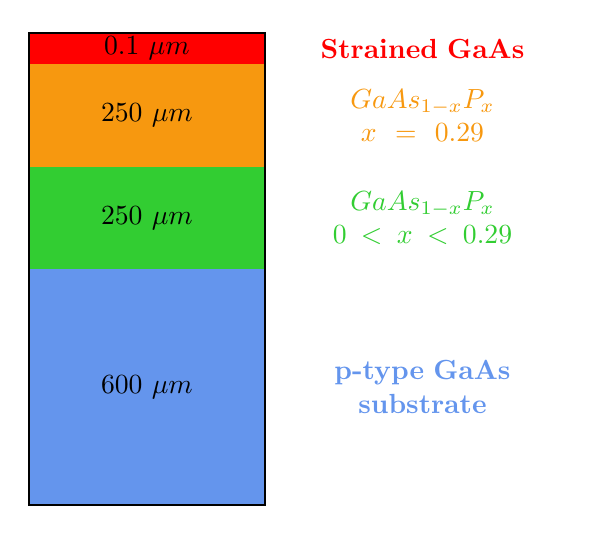
\begin{tikzpicture}
	    \tikzstyle{explain} = [align=center] 
	    \centering
	    \fill [CornflowerBlue] (0, 0) rectangle (3, 3);
	    \node at (3/2, 3/2) {\bm{$600 \ \mu m$}};
	    \node [explain, CornflowerBlue, text width=3.4 cm] at (5, 3/2) {\textbf{p-type GaAs substrate}};
	    \fill [LimeGreen] (0, 3) rectangle (3, 3+1.3);
	    \node at (3/2, 3 + 1.3/2) {\bm{$250 \ \mu m$}};
	    \node [explain, LimeGreen, text width=3.5 cm] at (5, 3+1.3/2) {\bm{$GaAs_{1-x}P_x$} \\ \bm{$0 < x < 0.29$}};
	    \fill [YellowOrange] (0, 3+1.3) rectangle (3, 3+1.3+1.3);
	    \node at (3/2, 3 + 1.3 + 1.3/2) {\bm{$250 \ \mu m$}};
	    \node [explain, YellowOrange, text width=3.5 cm] at (5, 3+1.3+1.3/2) {\bm{$GaAs_{1-x}P_x$} \\ \bm{$x = 0.29$}};
	    \fill [Red] (0, 3+1.3+1.3) rectangle (3, 6);
	    \node at (3/2, 3 + 1.3 + 1.3 + 0.4/2) {\bm{$0.1 \ \mu m$}};
	    \node [explain, Red, text width=3.5 cm] at (5, 3+1.3+1.3+0.4/2) {\textbf{Strained GaAs}};
	    \draw [thick] (0, 0) rectangle (3, 6);
	    \label{fg:excitation-a}
	\end{tikzpicture}
    \end{subfigure}
    \hfill
    \begin{subfigure}[b]{0.49\textwidth}
	\centering
	\begin{tikzpicture}
	    \begin{axis}[axis lines=middle,
		xmin=0, xmax=8,
		ymin=0, ymax=7,
		xlabel={\large $m_j$},
		ylabel={\large$E$},
		xlabel style={above},
		xtick=\empty,
		ytick=\empty,
		]
		\draw [/pgfplots/every inner y axis line, draw=black] (6.5,0) -- (6.5, \pgfkeysvalueof{/pgfplots/ymax}) node [below right] {\large J}; 
		\draw [draw=Violet, line width=2pt] (1.25,\yone) -- (2.25, \yone) node [midway, below, Violet] {\textbf{-1/2}};
		\draw [draw=Violet, line width=2pt] (4.25,\yone) -- (5.25, \yone) node [midway, below, Violet] {\textbf{+1/2}};
		\draw [draw=OliveGreen, line width=2pt] (0.5,\ytwo) -- (1.5, \ytwo) node [midway, below, OliveGreen] {\textbf{-3/2}};
		\draw [draw=OliveGreen, line width=2pt] (2,\ytwo-0.5) -- (3, \ytwo-0.5) node [midway, below, OliveGreen] {\textbf{-1/2}};
		\draw [draw=OliveGreen, line width=2pt] (3.5,\ytwo-0.5) -- (4.5, \ytwo-0.5) node [midway, below, OliveGreen] {\textbf{+1/2}};
		\draw [draw=OliveGreen, line width=2pt] (5,\ytwo) -- (6, \ytwo) node [midway, below, OliveGreen] {\textbf{+3/2}};
		\draw [draw=Blue, line width=2pt] (2,\ythree) -- (3, \ythree) node [midway, above, Blue] {\textbf{-1/2}};
		\draw [draw=Blue, line width=2pt] (3.5,\ythree) -- (4.5, \ythree) node [midway, above, Blue] {\textbf{+1/2}};
		\node [Violet, right] at (6.7, \yone-0.1) {\large\bm{$P_{1/2}$}};
		\node [OliveGreen, right] at (6.7, \ytwo-0.1) {\large\bm{$P_{3/2}$}};
		\node [Blue, right] at (6.7, \ythree-0.1) {\large\bm{$S_{1/2}$}};

		\draw [-stealth, Red, line width=2pt] (1, \ytwo) -- (2.5, \ythree) node [above, midway, sloped] {\bm{$\sigma^+$}};
		\draw [-stealth, YellowOrange, line width=2pt] (5.5, \ytwo) -- (4, \ythree) node [above, midway, sloped] {\bm{$\sigma^-$}};
	    \end{axis}
	\end{tikzpicture}
	\label{fg:excitation-b}
    \end{subfigure}
    \caption{Strained GaAs}
\end{figure}

%%%%%%%%%%%%%%%%%%%%%%%%%%%%%%%%%%%%%%%%%%%%%%%%
\subsection{Polarization Control}
\begin{figure}[h]
    \includegraphics[width=\linewidth]{injector}
\end{figure}

\begin{figure}[h]
    \begin{tikzpicture}
	\begin{scope}
	    \node[anchor=south west, inner sep=0] (image) at (0, 0)
	    {\includegraphics[width=\linewidth]{laser_table}};
	    \begin{scope}[x={(image.south east)},y={(image.north west)}]
	    \end{scope}
	\end{scope}
    \end{tikzpicture}
\end{figure}

%%%%%%%%%%%%%%%%%%%%%%%%%%%%%%%%%%%%%%%%%%%%%%%%
\subsection{Beam Modulation}

%%%%%%%%%%%%%%%%%%%%%%%%%%%%%%%%%%%%%%%%%%%%%%%%
\subsection{Target}

%%%%%%%%%%%%%%%%%%%%%%%%%%%%%%%%%%%%%%%%%%%%%%%%
\subsection{Magnets}

%%%%%%%%%%%%%%%%%%%%%%%%%%%%%%%%%%%%%%%%%%%%%%%%
\subsection{HRS}

%%%%%%%%%%%%%%%%%%%%%%%%%%%%%%%%%%%%%%%%%%%%%%%%
\subsection{Detector}
